\chapter{Genetikus algoritmus}

Az élővilág egyik alappillére a szaporodás, ami biztosítja a fajok túlélését hosszú távon. Az evolúciós törvényeket betartva azok a fajok maradnak fenn legtovább, akik jobban tudtak alkalmazkodni a környezetükhöz; a vadonban a legnagyobb, legerősebb, legtalálékonyabb fajok vannak előnyben, így szaporodáskor is nagyobb esélyük van pont ezeket a géneket továbbadni. Minél jobb génekkel rendelkezik egy élőlény, annál életrevalóbb utódjai lesznek, és ezzel növelik az egész faj esélyét a túlélésre. R. A. Fisher\footnote{Ronald Aylmer Fisher (1890--1962) brit statisztikus, genetikus} még az 1950-es években fejlesztette ki azt a matematikai modellt, amelyet a mai formába John Henry Holland\footnote{John Henry Holland (1929--2015) amerikai számítástechnika és pszichológia professzor} ültetett át, és manapság genetikus algoritmusnak \index{genetikus algoritmus} hívunk \parencite{holland2012}.

\section{A genetikus algoritmus alapjai}

A genetikus algoritmus populációját olyan egyedek (ún. kromoszómák) alkotják, amelyek géneket hordoznak magukban. A gének száma megegyezik az optimalizációs probléma dimenzionalitásával, vagyis általános esetben $n$ darab génnel rendelkezik az egyed. Minden kromoszóma a keresési mezőben potenciális megoldás lehet, így mindre ki tudjuk számolni a kritériumfüggvény értékét, ami az egyed alkalmasságát jelenti. A genetikus algoritmus célja, hogy az egyedek génjeit úgy változtatja meg, hogy azok alkalmassági értékei a lehető legjobbak legyenek, így megtalálva az optimális értéket. A kromoszómák génjeit \textit{genetikus műveletek} \index{genetikus műveletek} segítségével lehet változtatni.

\section{A genetikus műveletek}

Ebben a részben különféle genetikus műveleteket mutatunk be.

\subsection{Kiválasztás}

Általános esetben a populációt $N$ darab kromoszóma alkotja, melyeknek az alkalmassági értékein kell javítani. A genetikus elméletet követve a legjobb génekkel rendelkező egyedeknek kell utódokat létrehozniuk annak érdekében, hogy az egész populáció génállományát erősítsék. Tehát minden új ciklusban (generációban) meg kell ismételni a genetikus műveleteket. Egyszerre két egyedet kell kijelölni úgy, hogy a kiválasztás valószínűsége egyenesen arányos legyen az egyed alkalmasságával.

Egy efféle algoritmus a \textit{rulettkerék kiválasztás} \index{rulettkerék kiválasztás}, ami minden egyednek biztosít egy mezőt a keréken, de a mező szélessége egyenesen arányos az egyedhez rendelt kiválasztási valószínűséggel. Első gondolatra ez nem is tűnik rossz megoldásnak, másrészt viszont olyan mellékhatás léphet fel, ami szuper-egyedeket generál: így nem tudjuk biztosítani a globálisan elérhető optimumot, ha a szuper-egyed egy lokális optimumban akad meg. Ez a szuper-egyed később magához vonza a többi egyedet is, így a globális optimumot mind elkerüli \parencite{kanovic2017}.

Ahhoz, hogy ne favorizáljunk túl bizonyos géneket, rang alapú rendszert kell bevezetni, ahol az egyedek az alkalmassági értékük alapján vannak sorrendbe állítva, és $1$-től $N$-ig terjedő számmal vannak megjelölve. Tehát egy nagyon jó génekkel ellátott egyed és egy kevésbé jó géneket hordozó egyed között sokkal kisebb ez esetben a különbség.

\subsection{Keresztezés}

A kiválasztott egyedek képezik azt a halmazt, amiből majd kikerülnek a jövendőbeli szülők. Az utódok keresztezés útján jönnek létre, és így örökölnek bizonyos tulajdonságokat a felmenőiktől. Ez a művelet változtatja a populáció helyzetét, vagyis egyenes úton manipulálja a kromoszómák génszerkezetét.

A keresztezést többféle módon lehet kivitelezni:

\begin{itemize}
    \item binárisan kódolt gének uniform keresztezése (\ref{fig:keresztezes} ábra)
    
Két szülőtől két utód jön létre olyan módon, hogy egy véletlenszerűen generált bit-maszkot használva keverjük össze a szülők génjeit. (Az első utód az első szülőtől kap egy gént, ha a bit-maszkban 0 szerepel, ha pedig 1-es, akkor a második szülőtől. A második utód pedig ellenkező logikával kapja meg a génjeit).

\begin{figure}
    \centering
    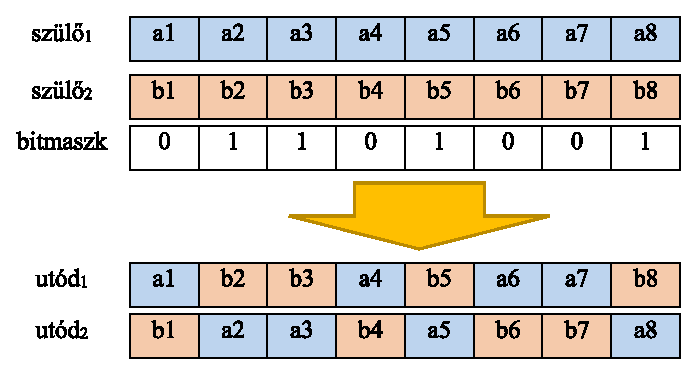
\includegraphics[width=0.75\textwidth]{keresztezes}
    \caption{Bináris uniform keresztezés \parencite{kanovic2017}}
    \label{fig:keresztezes}
\end{figure}

    \item reális számokkal kódolt gének aritmetikai keresztezése
    
A reális számoknál is hasonló keresztezés által születnek meg az utódok. A szülők ($x_1$ és $x_2$) génjeinek lineáris kombinációja alkotja az utódok génjeit (\ref{eq:keresztezes} képlet).

\begin{equ}[!ht]
  \begin{equation}
    \begin{aligned}
      x_1^0 &= a \cdot x_1 + (1-a) \cdot x_2 \\
      x_2^0 &= a \cdot x_2 + (1-a) \cdot x_1
    \end{aligned}
  \end{equation}
  \caption{\label{eq:keresztezes}}
\end{equ}

Ebben az esetben az a paraméter egy véletlenszerű szám 0 és 1 között, ami megfelel az előző példában szereplő bit-maszknak.
\end{itemize}

\subsection{Mutáció}

Mint ahogy az a természetes evolúcióban is jelentkezik, a gének időszakonként mutálódnak, így egy olyan populáció jön létre, amely nagyon kis mértékben eltér az előző generációtól. Ez azért fontos, mert ezek a kis mutációk jelentik azt a génbeli sokszínűséget, ami ellenállóbbá teszi az egyedeket (pl. kórokozók ellen).

A genetikus algoritmusban azért van szükség mutációra, hogy ne részesítsünk előnyben bizonyos egyedeket, amik így nem válnak szuper-egyedekké. Habár ezt a genetikus műveletet elenyésző számú egyeden végzik el, mégis gyorsabb konvergenciót eredményez, mintha mutáció nélkül zajlott volna az algoritmus \parencite{kanovic2017}.

Valós számok esetében a mutáció a következőképp végezhető el:

\begin{itemize}
    \item a génhez tartozó valós számot egy véletlenszerű valós számmal váltjuk fel (legdrasztikusabb hatást vált ki),
	\item nullához közeli valós szám hozzáadása vagy kivonása, vagy
	\item egyhez közeli valós számmal való szorzás.
\end{itemize}

Miután befejeztük a genetikus műveleteket, el kell dönteni, hogy mely egyedek kerülnek be a következő generációba. A legegyszerűbb módszer az újonann kapott egyedeket átmenti a következő generációba, míg az összes szülőt kitörli a keresési mezőből. Ezzel az a gond, hogy egyes rendkívül jó génekkel rendelkező szülő le lesz cserélve egy estleges kevésbé jó utódra. Az ilyen probléma kiküszöbölésére alkalmazzák az \textit{elitizmus} \index{elitizmus} elvét, miszerint bizonyos kritériumoknak megfelelő szülő át lesz mentve a következő generációra és potenciálisan lehet még utódja. Ez segíti az algoritmus konvergencióját, de elővigyázatosan kell kiválasztani azt a bizonyos elit kritériumot; különben létrejön egy \textit{szuper-egyed} \index{szuper-egyed}, ami nem minden esetben a globális optimumot mutatja \parencite{kanovic2017}.

\section{A genetikus algoritmus elemzése}

A genetikus algoritmus empírikus analíziseként a szakirodalom tesztfüggvények elemzését ajánlja \parencite{kanovic2017}. Ebben a dolgozatban bemutató jelleggel csak egy ún. Rastrigin-féle tesztfüggvény \index{Rastrigin-függvény} elemzése kerül elemzésre.

A Rastrigin-féle függvény érdekessége, hogy sok lokális minimuma van, és a \ref{eq:rastrigin} képlettel van definiálva. A függvény háromdimenziós grafikonja a \ref{fig:rastrigin3d} ábrán megtekinthető, valamint a függvény x-y síkra tett vetülete (\ref{fig:rastriginxy} ábra).

\begin{equ}[!ht]
  \begin{equation}
    f(x) = 10n + \sum_{i=1}^{n} (x_i^2 - 10 \cos(2 \pi x_i))
  \end{equation}
  \caption{\label{eq:rastrigin}}
\end{equ}

Általános esetben a függvény optimális értéke: $f(x^*)=0$, $x^*=[0,0,...,0]$, míg kétdimenziós probléma esetében ($n=2$): $f(x^*)=0$, $x^*=[0,0]$.

\begin{figure}
    \centering
    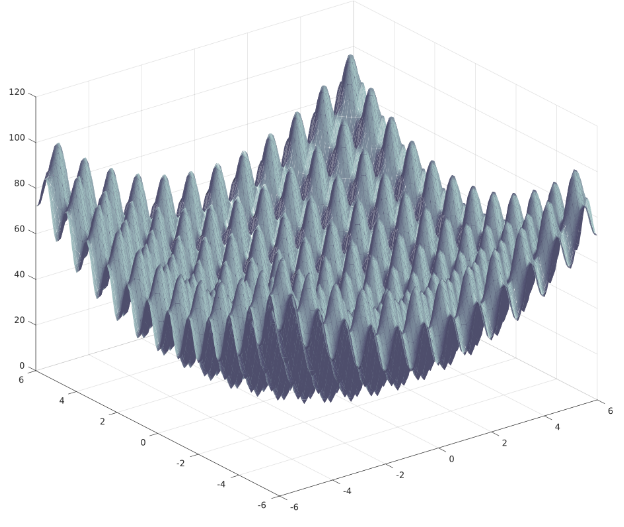
\includegraphics[width=0.8\textwidth]{rastrigin3d}
    \caption{Rastrigin-függvény grafikonja}
    \label{fig:rastrigin3d}
\end{figure}

\begin{figure}
    \centering
    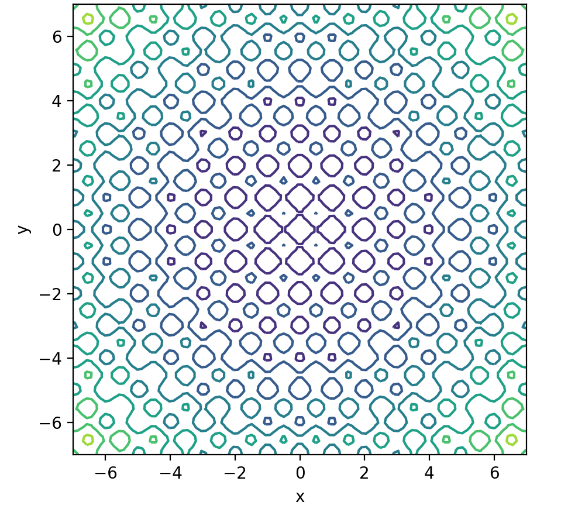
\includegraphics[width=0.8\textwidth]{rastriginxy}
    \caption{Rastrigin-függvény x-y vetülete}
    \label{fig:rastriginxy}
\end{figure}

A számításokat a \textit{Matlab} szoftvercsomag \textit{Optimization Toolbox} \parencite{matlab2016} moduljával végeztem. Négy különböző környezetben zajlott a számítás, más-más paraméterek mellett (generációszám és populációszám).

\linespread{1}
\begin{lstlisting}[language=Matlab, caption={A Rastrigin-függvény kódja}, captionpos=b]
function v = rastrigin(x)
	A = 10;
	s = sum(x.*x - A * cos(2*pi*x));
	v = A * length(x) + s;
end
\end{lstlisting}

A kísérletet százszoros megismétlése után születtek meg az eredmények, melyek a \ref{tab:genresult} táblázatban találhatók. Mindemellett az egyedek kezdőpozíciói elrendezettsége kétféle módon lett meghatározva: uniform elrendezettség (zöld), nem uniform elrendezettség (kék).

\begin{table}
    \centering
    \begin{tabular}{|m{0.5cm}|m{2.5cm}|m{2.5cm}|m{8cm}|}
    \hline
    \# & populációszám & generációszám & eredmények \\ \hline
    \hline
    K1 & 25 & 200 & 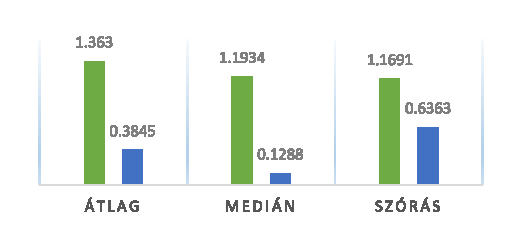
\includegraphics{gen1} \\ \hline
    K2 & 25 & 400 & 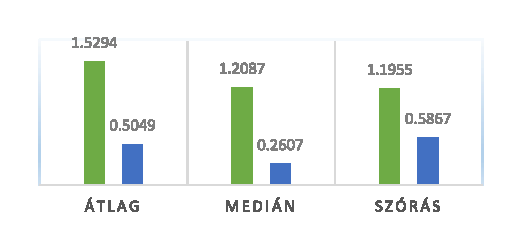
\includegraphics{gen2} \\ \hline
    K3 & 100 & 200 & 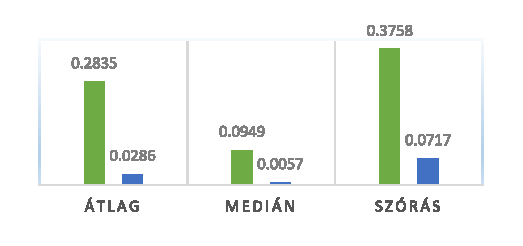
\includegraphics{gen3}	\\ \hline
    K4 & 200 & 200 & 
\includegraphics{gen4} \\ \hline
    \end{tabular}
    \caption{A Rastrigin-függvény elemzésének az eredményei}
    \label{tab:genresult}
\end{table}

Az eredmények alapján megállapíthatjuk, hogy a generáció számának a növelésével nem javult az eredményünk pontossága, míg a populáció számának a növelése nagyban hozzájárult a jobb eredményhez. A genetikus algoritmusnál a populáció számának a növelése drasztikusan lassítja az optimalizációs folyamatot, így a probléma sajátosságaihoz képest kell eldönteni, hogy gyors és kevésbé pontos eredményt kapunk, vagy lassú de pontosabb eredményt.

A legérdekesebb eredmények viszont az egyedek kezdőpozícióinak a változtatásakor születtek. Minden esetben jobb eredményt ért el az algoritmus, amikor a keresési mezőn nem egyenletesen (\ref{fig:uniform} ábra), hanem tömbben (\ref{fig:notuniform} ábra) helyezte el az egyedeket.

\begin{figure}
    \centering
    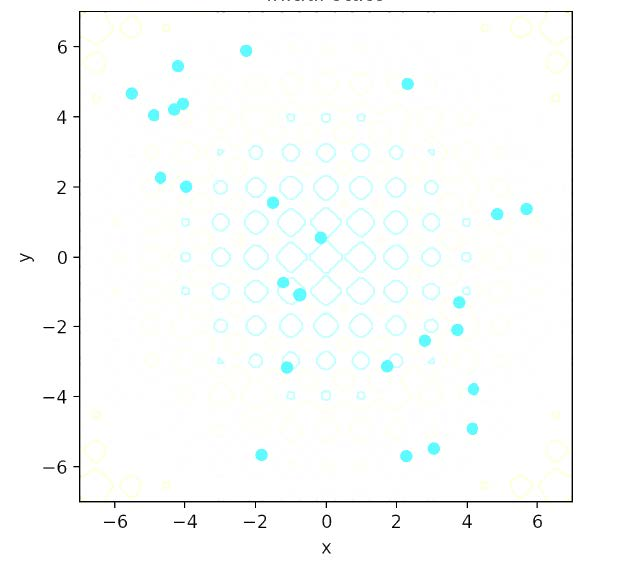
\includegraphics[width=0.7\textwidth]{uniform}
    \caption{Részecskék uniform kezdőpozíciói}
    \label{fig:uniform}
    \centering
    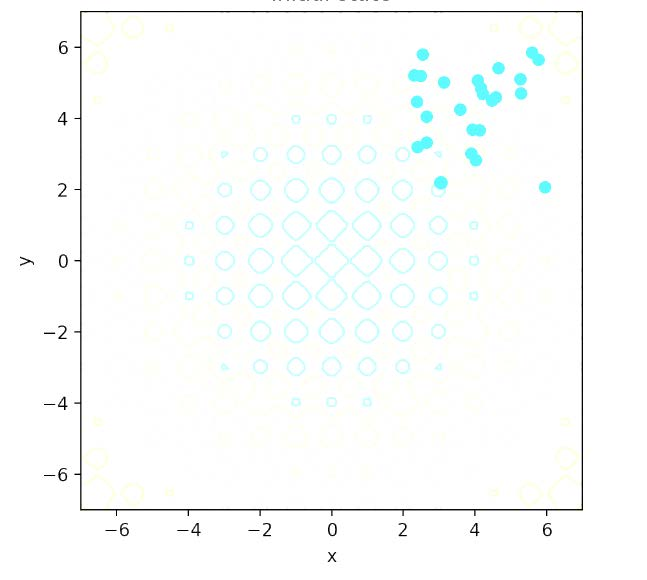
\includegraphics[width=0.7\textwidth]{notuniform}
    \caption{Részecskék nem-uniform kezdőpozíciói}
    \label{fig:notuniform}
\end{figure}

Az eredmények függvényében megállapítható, hogy a genetikai algoritmus jobban teljesít, ha kevesebb egyed nagyobb koncentrációban jelenik meg a keresési mezőn. A konkrét problémára levetítve ez jobb irányelvnek bizonyult, de más problémák esetében javasolt a paraméterek és a kezdőpozíció finomhangolása.

\section{A genetikus algoritmus felhasználási területei}

A genetikus algoritmus egy megbízható és állóképes algoritmus, mint amilyen a természetes evólúció is, amelyről modellezték. Rendkívűl széleskörű a használata: a matematikától kezdve, az egészségügyön át, a különböző mérnöki szakirányzatokig. A genetikus műveletek többféle módon való értelmezése különböző előnyöket ad a genetikus algoritmus felhasználásának más és más szakterületen: kombinatorikus problémák megoldása, képfeldolgozás, mesterséges neuronhálózatok és más gépi tanulási technikák \parencite{kanovic2017}.
